\documentclass[12pt,titlepage]{book}
\usepackage[margin=0.9in]{geometry} 
\usepackage{amsmath,amsthm,amssymb,graphicx,mathtools,tikz,hyperref}
\usepackage{pgfplots}
\usepackage{xcolor}
\newcommand{\redp}[1]{\textcolor{red}{#1}}
\newcommand{\bluep}[1]{\textcolor{blue}{#1}}
\newcommand{\tealp}[1]{\textcolor{teal}{#1}}
\usepackage{tcolorbox}
\newtcolorbox{mybox}{colback=red!5!white,colframe=red!75!black,fonttitle=\bfseries,title=Box}
\newtcolorbox{qt}{colback=orange!5!white,colframe=orange!75!white}
\usetikzlibrary{patterns,hobby}
\numberwithin{equation}{section}
\usepackage{wrapfig}
\usepackage{indentfirst}
\usepackage{ragged2e}
\RaggedRightParindent = 24 pt
\setlength{\parskip}{0.8em}
\renewcommand{\baselinestretch}{1.5}
\usepackage[noline]{algorithm2e}
\SetAlFnt{\footnotesize}
\usepackage{graphicx}
\usepackage{titling}
\renewcommand\maketitlehooka{\null\mbox{}\vfill}
\renewcommand\maketitlehookd{\vfill\null}
\usepackage{tocloft}
\renewcommand\cftsecafterpnum{\vskip6pt}
\usepackage{makeidx}
\makeindex
\usepackage{mdframed}
\newenvironment{que}
    { \begin{mdframed}[backgroundcolor=green!20] \textbf{$\Delta$ Question} \\}
    {  \end{mdframed}}
\newenvironment{thm}
    { \begin{mdframed}[backgroundcolor=orange!20] \textbf{$\Delta$ Theorem} \\}
    {  \end{mdframed}}
\newenvironment{defi}
    { \begin{mdframed}[backgroundcolor=red!10] \textbf{$\Delta$ Definition} \\}
    {  \end{mdframed}}
\newenvironment{lemma}
    { \begin{mdframed}[backgroundcolor=gray!10] \textbf{$\cdot$ Lemma} \\}
    {  \end{mdframed}}
\newenvironment{example}
    { \begin{mdframed}[backgroundcolor=white!10] \textbf{$\cdot$ Example} \\}
    {  \end{mdframed}}
\usepackage{graphicx}
\usepackage{float}
\usepackage{longtable}
\usepackage{tikz}
\usepackage{esint}
\usepackage{CJKutf8}
\usepackage{oubraces}

\title{Quantum Field Theory for Educated Dummies}
\author{Sizhe Liu\\University of Illinois at Urbana-Champaign }
\date{Version 1.0}

\pgfplotsset{compat=1.15}

\begin{document}

\maketitle

\chapter{Foundations}
\section{Natural Units and Dimensions}
Convenient systems of units start with arbitrary definitions for units of certain fundamental. quantities and derive the remaining units from laws of nature. To see how this works, assume we know three basic laws of nature and we want to devise a system of units from scratch. We will do this first for the cgs system and then for natural units.
The three lawas are:
\begin{qt}
\begin{itemize}
    \item The distance $L$ traveled by a photon is the speed of light multiplied by its time of travel. $L=c t$
    \item The energy of a massive particle is equal to its mass (at rest) $m$ times the speed of light squared. $E=mc^2$
    \item The energy of a photon is proportional to its frequency $f$. The constant of proportionality is Planck's constant $h . E=h f$ or re-expressed as $E=\hbar \omega$
\end{itemize}
\end{qt}
In natural units:\redp{the $c$ and $\hbar$ are dimensionless and equal to 1. The unit for energy is $MeV$}.

\section{Notation}
We shall use a notation defining \textbf{contravariant components $x^{\mu}$ of the $4 \mathrm{D}$ position vector} as $3 \mathrm{D}$ Cartesian coordinates $X_{i}$ plus $c t$ (see Appendix $\bar{A}$ if you are not comfortable with this), i.e.,
\begin{equation}
x^{\mu}=\left[\begin{array}{l}
{x^{0}} \\
{x^{1}} \\
{x^{2}} \\
{x^{3}}
\end{array}\right]=\left[\begin{array}{l}
{c t} \\
{X_{1}} \\
{X_{2}} \\
{X_{3}}
\end{array}\right]=\left[\begin{array}{l}
{c t, X_{i}}
\end{array}\right]^{T}
\end{equation}
From special relativity, we know the differential proper time passed on an object (with $c=1$ ) is
\begin{equation}
(d \tau)^{2}=(d t)^{2}-d X_{1} d X_{1}-d X_{2} d X_{2}-d X_{3} d X_{3}
\end{equation}
If we define \textbf{covariant components} of the 4D position vector as
\begin{equation}
x_{\mu}=\left[\begin{array}{l}
{x_{0}} \\
{x_{1}} \\
{x_{2}} \\
{x_{3}}
\end{array}\right]=\left[\begin{array}{c}
{t} \\
{-X_{1}} \\
{-X_{2}} \\
{-X_{3}}
\end{array}\right]=\left[t,-X_{i}\right]^{T}
\end{equation}
then
\begin{equation}
(d \tau)^{2}=d x^{0} d x_{0}+d x^{1} d x_{1}+d x^{2} d x_{2}+d x^{3} d x_{3}=d x^{\mu} d x_{\mu}
\end{equation}
Using metric tensor $g_{\mu\nu}$, we have the following relation:
\begin{equation}
x_{\mu}=g_{\mu \nu} x^{\nu}=\left[\begin{array}{cccc}
{1} & {0} & {0} & {0} \\
{0} & {-1} & {0} & {0} \\
{0} & {0} & {-1} & {0} \\
{0} & {0} & {0} & {-1}
\end{array}\right]\left[\begin{array}{c}
{x^{0}} \\
{x^{1}} \\
{x^{2}} \\
{x^{3}}
\end{array}\right]
\end{equation}
\redp{The inverse of $g_{\mu\nu}$, $g^{\mu\nu}$, has the exact same form.}Thus,
\begin{equation}
(d \tau)^{2}=g_{\mu v} d x^{\mu} d x^{v}=g^{\mu v} d x_{\mu} d x_{v}
\end{equation}
\begin{qt}
Partial derivative w.r.t. $x^{\mu}$ and $x_{\mu}$ are:
\begin{equation}
\partial_{\mu}=\frac{\partial}{\partial x^{\mu}}=\left(\frac{\partial}{\partial t}, \frac{\partial}{\partial x^{i}}\right)^{T}=\left(\frac{\partial}{\partial t} \cdot \frac{\partial}{\partial X_{i}}\right)^{T}
\end{equation}
and
\begin{equation}
\partial^{\mu}=\frac{\partial}{\partial x_{\mu}}=\left(\frac{\partial}{\partial t}, \frac{\partial}{\partial x_{i}}\right)^{T}=\left(\frac{\partial}{\partial t},-\frac{\partial}{\partial X_{i}}\right)^{T}
\end{equation}
\end{qt}
For a matrix, we can raise the index as
\begin{equation}
M^{\mu \nu}=g^{\mu \alpha} g^{\nu \beta} M_{\alpha \beta}
\end{equation}
\section{Review of Variational Methods}
Recall also, that given the Lagrangian, we could find the Hamiltonian $H,$ via the Legendre transformation (employing a Cartesian system where $x^{i}=x_{i}$ and $p^{i}=p_{i}$),
\begin{equation}
H=p_{i} \dot{x}^{i}-L, \quad \text { where } p_{i}=\frac{\partial L}{\partial \dot{x}^{i}}=m \dot{x}^{i}\left(=p^{\prime} \text { for Cartesian system }\right)
\end{equation}
$p_{i}$ is the conjugate, or canonical, momentum of $x$ '. (Note that a contravariant component in the denominator is effectively equivalent to a covariant component in the entire entity, and vice versa.) Hence, we can define:
\begin{qt}
\textbf{First quantization}

Keeping the classical Hamiltonian and, changing Poisson brackets to commutators, we could just as readily have used the Lagrangian L, or the equations of motion instead.
\end{qt}
\subsection{Classical Field Theory}
From particle theory to field theory, we have the following things changed:
\begin{qt}
$$L, H, e t c \rightarrow \mathcal{L}, \mathcal{H},$$ 
\[
x^{i}(t) \rightarrow \phi^{r}\left(x^{\mu}\right)
\]
$$t \rightarrow x^{\mu}$$
\end{qt}
Classical field theory is analogous in many ways to classical particle Lagrangian $L$, we have the Lagrangian density $\mathcal{L}$. Instead of time $t$ as an independent variable, we have $x^{\mu}=x^{0}, x^{1}, x^{2}, x^{3}=t, {x^{i}}$ as independent variables. Instead of a particle described by $x^{i}(t),$ \textbf{we have a field value described by $\phi(x^{\mu})$, where $r$ designates different field types, or possibly, different spatial components of the same vector field.}
\begin{qt}
The Euler-Lagrange equation for fields becomes
\begin{equation}
\frac{\partial}{\partial x^{\mu}}\left(\frac{\partial \mathcal{L}}{\partial \phi^{r}, \mu}\right)-\frac{\partial \mathcal{L}}{\partial \phi^{r}}=0
\end{equation}
and
\begin{equation}
\mathcal{H}=\pi_{r} \dot{\phi}^{r}-\mathcal{L}, \quad \text { where } \pi_{r}=\frac{\partial \mathcal{L}}{\partial \dot{\phi}^{r}}
\end{equation}
with $\pi_r$ being the conjugate momentum density of the field $\phi^r$. And the action is
\begin{equation}
S=\int_{T} \int_{V} \mathcal{L}\left(\phi, \phi_{,\mu}\right) d^{3} \mathbf{x} d t=\int_{\Omega} \mathcal{L}\left(\phi, \phi_{, \mu}\right) d^{4} x
\end{equation}
\end{qt}
\subsection{Key concepts in field theory}
For fields
\begin{equation}
\frac{\partial \phi}{\partial t}=\frac{d \phi}{d t}=\dot{\phi}
\end{equation}
This is generally not true for other quantities. For fields, 
\begin{equation}
\frac{d \phi}{d t}=\frac{\partial \phi}{\partial x^{\prime}} \frac{d x^{\prime}}{d t}+\frac{\partial \phi}{\partial t} \frac{d t}{d t}
\end{equation}
\redp{where $\frac{dx^i}{dt}$ are equal to zero}.

For a single particle, particle position coordinates are the generalized coordinates and particle momentum components are its conjugate momenta. For fields, each field is itself a generalized coordinate and each field has its own conjugate momentum (density). As noted, this field conjugate momentum (density) is different from the physical momentum (density) that the field possesses.

For conjugate and physical momentum densities, we have the following density relation
$$
p_{t}=\frac{\partial L}{\partial \dot{x}^{t}} \quad \frac{\text { for small particle in medium, }}{\text { divide by particle volume }}, \quad \mathcal{R}_{i}=\frac{\partial \mathcal{L}}{\partial \dot{x}^{i}}
$$
We note carefully that our $x^i$ here is the position coordinate of a point fixed relative to the field and thus is time dependent. Further, the total derivative $\dot{x}^i$ equals the partial derivative w.r.t. time, since $x^i$ in the present case is only a function of time. Now take the \redp{conjugate momentum density relation for relativistic fields},
$$
\pi_{r}=\frac{\partial \mathcal{L}}{\partial \dot{\phi}^{r}}
$$
and
$$
\frac{\mathcal{R}_{i}}{\pi_{r}}=\frac{\partial \mathcal{L} / \partial \dot{x}^{i}}{\partial \mathcal{L} / \partial \dot{\phi}^{r}}=\frac{\partial \dot{\phi}^{r}}{\partial \dot{x}^{\prime}}=\frac{\partial \phi^{r} / \partial t}{\partial x^{i} / \partial t}=\frac{\partial \phi^{r}}{\partial x^{i}} \quad \rightarrow \quad \mathcal{R}_{i}=\pi_{r} \frac{\partial \phi^{r}}{\partial x^{i}} \quad \rightarrow \quad \mathcal{R}^{i}=-\pi_{r} \frac{\partial \phi^{r}}{\partial x^{i}}
$$
The partial derivative of $\phi^{r}$ with respect to either of our definitions of $x^{i}$ (time dependent as the moving position of a point fixed to the field, or time independent as coordinates fixed in space) is the same because by definition, partial derivative means we hold everything else here constant, Thus, the above relation holds in field theory when we consider the $x^{i}$ as independent variables (coordinates fixed in space).

The field equation (equations of motion) for relativistic fields keep the exact same form in any inertial frame of reference, i.e., they are \redp{Lorentz invariant}. Four scalars(world scalars) are \redp{invariant under a Lorentz transformation and look exactly the same to any observer.}
\begin{qt}
The mass $m$ in relativity of a free particle is four scalar, where $m^2=p^{\mu}p_{\mu}$.

Demanding that the Euler-Lagrange equation be Lorentz invariant, we know that, within that equation, $x^{\mu}$,$\phi^r$, and derivatives of $x^{\mu}$ are Lorentz covariant or invariant. \redp{So, in order for the whole equation to be Lorentz invariant, the Lagrangian density $\mathcal{L}$ must be invariant.}

Further, L, H, and $\mathcal{H}$ are not Lorentz scalars.
\end{qt}

\section{Schrodinger vs. Heisenberg Pictures}

\chapter{Scalars: Spin 0 Fields}
\section{Deducing Klein-Gordon Equation}
If we squared the operators in the original Schrodinger equation, we obtain
\begin{equation}
\left(i \hbar \frac{\partial}{\partial t}\right)\left(i \hbar \frac{\partial}{\partial t}\right) \phi=H^{2} \phi=\left(\mathbf{p}_{o p e r}^{2} c^{2}+m^{2} c^{4}\right) \phi
\end{equation}
which becomes
\begin{equation}
-\frac{\hbar^{2}}{c^{2}} \frac{\partial^{2}}{\partial t^{2}} \phi=\left(-\hbar^{2} \frac{\partial}{\partial X_{i}} \frac{\partial}{\partial X_{i}}+m^{2} c^{2}\right) \phi
\end{equation}
In a compact form, we have
\begin{equation}
-\frac{\partial}{\partial x^{0}} \frac{\partial}{\partial x_{0}} \phi=\left(\frac{\partial}{\partial x^{i}} \frac{\partial}{\partial x_{i}}+\frac{m^{2} c^{2}}{\hbar^{2}}\right) \phi
\end{equation}
where we define $\mu^2=\frac{m^{2} c^{2}}{\hbar^{2}}$. Re-arranging, we have the Klein-Gordon equation
\begin{qt}
    \begin{equation}
\left(\partial_{\mu} \partial^{\mu}+\mu^{2}\right) \phi=0
\end{equation}
The operation $\partial_{\mu} \partial^{\mu}=\partial^{\mu} \partial_{\mu}$ is called the \textbf{d'Alembertian} operator, and is the 4D Minkowski coordinates analogue of the 3D Laplacian operator of Cartesian coordinates.
\end{qt}
\subsection{The solutions to the Klein-Gordon Equation}
\begin{equation}
\phi(x)=\sum_{n=1}^{\infty} \frac{1}{\sqrt{2 V E_{n} / \hbar}}\left(A_{n} e^{-\frac{i}{\hbar}\left(E_{n} t-\mathbf{p}_{n} \cdot \mathbf{x}\right)}+\underbrace{B_{n}^{\dagger} e^{\frac{i}{\hbar}\left(E_{n} t-\mathbf{p}_{n} \cdot \mathbf{x}\right)}}_{\text {absent in NRQM }}\right)
\end{equation}
Because we are using the square of the relativistic Hamiltonian in RQM, \bluep{we get additional solutions of exponential form $+i(E_nt-\mathbf{p}_n\cdot\mathcal{x})/\hbar$ that also solve the relativistic Klein-Gordon equation}.

With an aim towards using natural units, we note the following relations, where wave number $k_{i}$ $=2 \pi / \lambda_{i}$ and we use the deBroglie relation $p^{i}=\hbar k^{i}$
\begin{qt}
    \begin{equation}
p_{\mu}=\left[\begin{array}{c}
{E / c} \\
{p_{i}}
\end{array}\right]=\left[\begin{array}{c}
{E / c} \\
{-p^{i}}
\end{array}\right]=\hbar k_{\mu}=\left[\begin{array}{c}
{\hbar \omega / c} \\
{-\hbar k^{\prime}}
\end{array}\right]
\end{equation}
in natural units
\begin{equation}
p_{\mu}=\left[\begin{array}{c}
{E} \\
{-p^{i}}
\end{array}\right]=k_{\mu}=\left[\begin{array}{c}
{\omega} \\
{-k^{i}}
\end{array}\right]
\end{equation}
\end{qt}
Recall the notation introduced in the previous chapter, we have
\begin{equation}
p x=p_{\mu} x^{\mu}=E t-p^{i} x^{i}=p^{\mu} x_{\mu}
\end{equation}
\begin{equation}
k x=k_{\mu} x^{\mu}=\omega t-k^{i} x^{i}=\frac{E t}{\hbar}-\frac{p^{i} x^{i}}{\hbar}=\frac{p_{\mu}}{\hbar} x^{\mu}
\end{equation}
In natural unit
\begin{equation}
E=\omega, \quad p_{i}=k_{i}, \quad p_{\mu}=k_{\mu}, \quad p x=k x
\end{equation}
\bluep{For free fields, a given wave with wave number vector $\mathbf{k}$ has a particular energy, and we can designate that energy via either $E_{\mathbf{k}} \text { or } \omega_{\mathbf{k}} .$ It is common practice for scalars to use $\mathbf{k} \text { (rather than } \mathbf{p})$ and $\mathbf{k}$ (rather than $E_{\mathbf{p}}$ or $E_{\mathbf{k}}$.)}

The Klein-Gordon equation solutions then become, in natural units
\begin{equation}
\phi(x)=\sum_{k} \frac{1}{\sqrt{2 V_{e l}}}\left(A_{k} e^{-i k x}+B_{k}^{\dagger} e^{i k x}\right)
\end{equation}
\begin{mybox}
In RQM, the solution $\phi$ is that of a general (sum of eigenstates) single particle state. Each eigenstate has mathematical form of
$$
\phi_{k, A}=\frac{e^{-i k x}}{\sqrt{V}}
$$
$$
\quad \phi_{\mathrm{k}, B^{\dagger}}=\frac{e^{i k x}}{\sqrt{V}}
$$
Each of these forms has what is called \textbf{unit norm}. That is, all such eigenstates are \textbf{orthonormal}:
\begin{equation}
\int \phi_{k, A}^{\dagger} \phi_{k^{\prime},A} d^{3} x=\frac{1}{V} \int e^{i k x} e^{-i k^{\prime} x} d^{3} x=\delta_{k k^{\prime}}
\end{equation}
Similar relations exist for $\phi_{k, B^{\dagger}}$.
\end{mybox}

\subsection{Deducing probability density in RQM}
Starting from the Klein-Gordon equation, first post-multiply it by $\phi^{\dagger}$, then subtract the complex conjugate equation post-multiplied by $\phi$,
\begin{equation}
\begin{array}{c}
{\left\{\frac{\partial^{2}}{\partial t^{2}} \phi=\left(\nabla^{2}-\mu^{2}\right) \phi\right\} \phi^{\dagger}} \\
{-\left\{\frac{\partial^{2}}{\partial t^{2}} \phi^{\dagger}=\left(\nabla^{2}-\mu^{2}\right) \phi^{\dagger}\right\} \phi}
\end{array}
\end{equation}
Since $\mu^{2} \phi^{\dagger} \phi-\mu^{2} \phi \phi^{\dagger}=0$, we obtain
\begin{equation}
i \frac{\partial}{\partial t}\left(\frac{\partial \phi}{\partial t} \phi^{\dagger}-\frac{\partial \phi^{\dagger}}{\partial t} \phi\right)=i \nabla \cdot\left((\nabla \phi) \phi^{\dagger}-\left(\nabla \phi^{\dagger}\right) \phi\right)
\end{equation}
where probability density and the probability current for a Klein-Gordon particle are
\begin{qt}
    \begin{equation}
\rho=j^{0}=i\left(\frac{\partial \phi}{\partial t} \phi^{\dagger}-\frac{\partial \phi^{\dagger}}{\partial t} \phi\right)
\end{equation}
and
\begin{equation}
\mathbf{j}=-i\left((\nabla \phi) \phi^{\dagger}-\left(\nabla \phi^{\dagger}\right) \phi\right) \quad j^{i}=-i\left(\phi_{,i} \phi^{\dagger}-\phi_{, i}^{\dagger} \phi\right)=i\left(\phi^{,i} \phi^{\dagger}-\phi^{\dagger, i} \phi\right)
\end{equation}
\end{qt}
Now we can define the \redp{4-currents} as
\begin{equation}
j^{\mu}=\left[\begin{array}{l}
{\rho} \\
{\mathbf{j}}
\end{array}\right]=\left[\begin{array}{l}
{\rho} \\
{j^{i}}
\end{array}\right]=\left[\begin{array}{l}
{j^{0}} \\
{j^{i}}
\end{array}\right]=i\left(\phi^{\mu} \phi^{\dagger}-\phi^{\dagger,\mu} \phi\right)
\end{equation}
The \redp{4D continuity equation} is then
\begin{qt}
    \begin{equation}
\frac{\partial j^{\mu}}{\partial x^{\mu}}=\partial_{\mu} j^{\mu}=j^{\mu}{ }_{,\mu}=0
\label{4d-continuity-eq}
\end{equation}
\end{qt}
(\ref{4d-continuity-eq}) tells us the important fact that \bluep{the 4-divergence of the 4-current of any conserved quantity is zero}.

\bluep{The total probability of unity is a relativistic invariant. Further $A_{k}$ here are constants that do not vary with frame.}\redp{So the probability of  finding any particular state is also independent of what frame the measurements are taken in.}

\subsection{Negative Energies in RQM}
If we apply traditional Hamiltonian operator $H$ as $i\partial/\partial t$ to $\phi_{\mathbf{k},B^{\dagger}}$:
\begin{equation}
i \frac{\partial \phi_{\mathbf{k}, B^{\dagger}}}{\partial t}=i \frac{\partial}{\partial t} \frac{e^{i k x}}{\sqrt{V}}=-\omega_{\mathbf{k}} \frac{e^{i k x}}{\sqrt{V}}=-\omega_{\mathbf{k}} \phi_{\mathbf{k}, B^{\dagger}}=E_{\mathbf{k}, B^{\prime}} \phi_{\mathbf{k}, B^{+}}
\end{equation}
Since $\omega_{\mathbf{k}}$ is always a positive number, we have states with \redp{negative energies in RQM, and we need QFT to solve this dilemma}. 

\section{Klein-Gordon Equation in Quantum Field Theory}

\chapter{Spinors: Spin 1/2 Fields}
\section{Dirac's Approach to RQM:}
Dirac's primary goal was a 1st order relativistic Schrodinger equation, and he postulated that if it existed, it must have the general form of 
\begin{equation}
i \frac{\partial}{\partial t}|\psi\rangle= H|\psi\rangle=(a \cdot \mathbf{p}+\beta m)|\psi\rangle
\label{1st-order-relativistic-SDE}
\end{equation}
In \ref{1st-order-relativistic-SDE}, $\mathbf{p}$ is particle three momentum (an operator in quantum theories), and the vector $\alpha$ and the scalar $\beta$ would have to be determined. Thus, the equation would be first order in the time derivative. To find $\alpha$ and $\beta$, Dirac reasoned that $H^{2}$ and $|\psi\rangle$ must also satisfy the usual relativistic energy momentum relation (and therefore the Klein-Gordon equation)
$$
-\frac{\partial^{2}}{\partial t^{2}}|\psi\rangle= H^{2}|\psi\rangle=\left(\mathbf{p}^{2}+m^{2}\right)|\psi\rangle
$$
Thus
$$
-\frac{\partial^{2}}{\partial t^{2}}|\psi\rangle= H^{2}|\psi\rangle=\left(\alpha_{i} p_{i}+\beta m\right)\left(\alpha_{j} p_{j}+\beta m\right)|\psi\rangle
$$
$$
=\left(\alpha_{i}^{2} p_{i}^{2}+\underbrace{\left(\alpha_{i} \alpha_{j}+\alpha_{j} \alpha_{i}\right)}_{\text {must }=0}p_{i}p_{j}+\underbrace{\left(\alpha_{i} \beta+\beta \alpha_{i}\right)}_{\text {must }=0} p_{i} m+\beta^{2} m^{2}\right)|\psi\rangle
$$
Therefore, $\alpha_{i}^{2}=1$ and $\beta^{2}=1$. In summary, we have anti-commutators relationship:
\begin{qt}
    \begin{equation}
\begin{aligned}
&\left[\alpha_{i}, \alpha_{j}\right]_{+}=\left[\alpha_{i}, \beta\right]_{+}=0 \quad i \neq j \quad \alpha_{1}, \alpha_{2}, \alpha_{3}, \beta \text { all anti-commute with each other, }\\
&\left(\alpha_{1}\right)^{2}=\left(\alpha_{2}\right)^{2}=\left(\alpha_{3}\right)^{2}=(\beta)^{2}=1 \text { (the identity matrix) }
\end{aligned}
\label{standard-condition}
\end{equation}
\end{qt}
\bluep{If $\alpha_{i}$ and $\beta$ were numbers they would have to commute and could not possibly anti-commute. Hence, they can only be matrices. since these matrices are operators operating on $|\psi\rangle,$ then $|\psi\rangle$ itself must be a multicomponent object (i.e., a column matrix, at least.)}. Use the relations above, one can show that the \redp{$\alpha$ and $\beta$ matrices are traceless, hermitian, have $\pm$ eigenvalues, and must have an even dimension of at least four}.

Square matrices in a 4D space must be  $4\mathrm{X} 4,$ and thus if $|\psi\rangle$ is a column matrix (a vector), it must have four components (a 4D vector). Take care to note the \bluep{4D space we are talking about here is not the four-dimensional physical space of relativity theory, but an abstract pace, often called \textbf{spinor space}}.
\subsection{Standard presentation}
Choosing the minimum dimension case (four), Dirac and Pauli came up with a set of matrices which solve all of the conditions in (\ref{standard-condition}):
$$
\beta=\left[\begin{array}{cccc}
{1} \\
{} & {1} \\
{} & {} & {-1} \\
{} & {} & {} & {-1}
\end{array}\right]
$$
$$
\alpha_{1}=\left[\begin{array}{cccc}
{}&{}&{}&{1} \\
{}&{}&{1} \\
{} & {1} \\
{1}
\end{array}\right] \quad \alpha_{2}=\left[\begin{array}{cccc}
{}&{}&{}&{-i} \\
{}&{}&{i} \\
{} & {-i} \\
{i}
\end{array}\right] \quad \alpha_{3}=\left[\begin{array}{cccc}
{}&{}&{1} \\
{}&{}&{}& {-1} \\
{1}\\
{}&{-1} 
\end{array}\right]
$$
which are commonly written using Pauli matrices
$$
\beta=\left[\begin{array}{cc}
{I} & {0} \\
{0} & {-I}
\end{array}\right] \quad \alpha_{1}=\left[\begin{array}{cc}
{0} & {\sigma_{1}} \\
{\sigma_{1}} & {0}
\end{array}\right] \quad \alpha_{2}=\left[\begin{array}{cc}
{0} & {\sigma_{2}} \\
{\sigma_{2}} & {0}
\end{array}\right] \quad \alpha_{3}=\left[\begin{array}{cc}
{0} & {\sigma_{3}} \\
{\sigma_{3}} & {0}
\end{array}\right]
$$
If we define \textbf{gamma matrices} or \redp{\textbf{Dirac matrices}} as:
\begin{equation}
\gamma^{0}=\beta \quad \gamma^{1}=\beta \alpha_{1} \quad \gamma^{2}=\beta \alpha_{2} \quad \gamma^{3}=\beta \alpha_{3}
\end{equation}
we find the \textbf{Hermiticity conditions} as
\begin{equation}
\gamma^{\mu \dagger}=\gamma^{0} \gamma^{\mu} \gamma^{0}
\end{equation}
\subsection{Dirac equation expressed with Dirac matrices}
Pre-multiplied $\beta$, Dirac's original $1^{st}$ order equation takes on the form
\begin{equation}
i \beta \frac{\partial}{\partial t}|\psi\rangle=\left(\beta \alpha_{i} p_{i}+\beta^{2} m\right) | \psi\rangle=\left(-i \gamma^{i} \frac{\partial}{\partial x^{i}}+m\right)|\psi\rangle
\end{equation}
or rearranged as what is formally called the \textbf{Dirac equation}:
\begin{equation}
\sum_{\eta=1}^{4}\left(\sum_{\mu=0}^{3} i\left(\gamma^{\mu}\right)_{\kappa \eta} \partial_{\mu}-m \delta_{\kappa \eta}\right)|\psi\rangle_{\eta}=0 \quad \kappa=1,2,3,4
\end{equation}
where we have written out the $4 \mathrm{X} 4$ spinor space indices in $\kappa$ and $\eta$. Note the Dirac equation is actually \textbf{four separate non-matrix equations}, one for each value of the index $\kappa$. And each of these equations entails a sum of matrix components (sum over $\mu$ ), each post multiplied by one of the four components (in $\eta$ index) of the column vector $|\psi\rangle$.
\begin{qt}
    The common way to write the Dirac equation is to hide the spinor space indices in $\kappa$ and $\eta$,
    \begin{equation}
\left(i \gamma^{\mu} \partial_{\mu}-m\right)|\psi\rangle= 0
\label{convenient-Dirac-eq}
\end{equation}
Another notation commonly used, which is the most streamlined of all, is
$$
\not \partial=\gamma^{\mu} \partial_{\mu} \quad \text { so, the Dirac equation } \rightarrow(i \not \partial-m)|\psi\rangle= 0
$$
\end{qt}
Also, $m \rightarrow \frac{m c}{\hbar} \quad$ in non-natural units in the Dirac equation.

\subsection{Solutions to the Dirac equation}
Write out (\ref{convenient-Dirac-eq}) fully as:
$$
i \gamma^{\mu} \partial_{\mu}|\psi\rangle= i\left(\gamma^{0} \partial_{0}+\gamma^{1} \partial_{1}+\gamma^{2} \partial_{2}+\gamma^{3} \partial_{3}\right)|\psi\rangle= m|\psi\rangle=
$$
$$
=i\left(\left[\begin{array}{cccc}
{\partial_{0}} & {0} & {\partial_{3}} & {\partial_{1}-i \partial_{2}} \\
{0} & {\partial_{0}} & {\partial_{1}+i \partial_{2}} & {-\partial_{3}} \\
{-\partial_{3}} & {-\partial_{1}+i \partial_{2}} & {-\partial_{0}} & {0} \\
{-\partial_{1}-i \partial_{2}} & {\partial_{3}} & {0} & {-\partial_{0}}
\end{array}\right]\right) \left| \begin{array}{l}
{\psi_{1}} \\
{\psi_{2}} \\
{\psi_{3}} \\
{\psi_{4}}
\end{array}\right\rangle=
m\left|\begin{array}{l}
{\psi_{1}} \\
{\psi_{2}} \\
{\psi_{3}} \\
{\psi_{4}}
\end{array}\right\rangle
$$
The Dirac equation solutions in the Dirac-Pauli (standard) representation are
\begin{qt}
$$
\left|\psi^{(1)}\right\rangle=\sqrt{\frac{E+m}{2 m}}\left(\begin{array}{c}
{1} \\
{0} \\
{\frac{p^{3}}{E+m}} \\
{\frac{p^{1}+i p^{2}}{E+m}}
\end{array}\right)  \underbrace{e^{-i p x}}_{\text {4D physical space part}}=u_1e^{-i p x}
$$
$$
\left|\psi^{(2)}\right\rangle=\sqrt{\frac{E+m}{2 m}}\left(\begin{array}{c}
{0} \\
{1} \\
{\frac{p^{1}-i p^{2}}{E+m}} \\
{\frac{-p^{3}}{E+m}}
\end{array}\right) e^{-i p x}=u_2e^{-i p x}
$$
$$
\left|\psi^{(3)}\right\rangle=\sqrt{\frac{E+m}{2 m}}\left(\begin{array}{c}
{\frac{p^{3}}{E+m}} \\
{\frac{p^{1}+i p^{2}}{E+m}}\\
{1} \\
{0} 
\end{array}\right) e^{i p x}=v_2e^{i p x}
$$
\begin{equation}
\left|\psi^{(4)}\right\rangle=\sqrt{\frac{E+m}{2 m}}\left(\begin{array}{c}
{\frac{p^{1}-i p^{2}}{E+m}}\\
{\frac{-p^{3}}{E+m}} \\
{0} \\
{1} 
\end{array}\right) e^{i p x}=v_1e^{i p x}
\label{four-spinors}
\end{equation}
\end{qt}
We have defined new symbols $u_{r}(\mathbf{p})$ and $v_{r}(\mathbf{p})(r=1,2),$ which are the column vectors multiplied by the constant shown, are functions only of $\mathbf{p}$ for a given $m(\text { since } E=\sqrt{\mathbf{p}^{2}+m^{2}}),$ and go by the name \textbf{spinors}, or \textbf{\redp{four-spinors}}. Note that \bluep{the particles represented by $|\psi^{(n)}\rangle$ are also often called spinors.}

\textbf{$u_{1}$ represents spin up, and $u_{2}$ represents spin down in the particle at-rest system. As you might expect, we will find the solutions containing $v_{r}(\mathbf{p})$ are associated with antiparticles; and those with $u_{r}(\mathbf{p}),$ with particles.}\redp{Take care to note the reverse order numbering on $v_{2,1}$ from $u_{1,2},$ which is customary.}

If we take \textbf{inner products of four spinors}, we have
$$
u_{1}^{\dagger}(\mathbf{p}) u_{1}(\mathbf{p})=\frac{E}{m}
$$
More generally
\begin{equation}
u_{\underline{r}L}^{\dagger}(\mathbf{p}) u_{\underline{r}}(\mathbf{p})=v_{\underline{r}}^{\dagger}(\mathbf{p}) v_{\underline{r}}(\mathbf{p})=\frac{E}{m}
\end{equation}
Where underline means no summation. Also, spinors are \textbf{orthogonal}
\begin{equation}
\begin{aligned}
&u_{r}^{\dagger}(\mathbf{p}) u_{s}(\mathbf{p})=v_{r}^{\dagger}(\mathbf{p}) v_{s}(\mathbf{p})=\frac{E}{m} \delta_{r s}\\
&u_{r}^{\dagger}(\mathbf{p}) v_{s}(-\mathbf{p})=0
\end{aligned}
\end{equation}
Therefore, the eigensolutions are also orthogonal
\begin{equation}
\left\langle\psi^{(m)} | \psi^{(n)}\right\rangle= 0 \text { for } m \neq n
\end{equation}
For example
$$
\left\langle\psi^{(1)} | \psi^{(3)}\right\rangle=\int u_{1}^{\dagger}(\mathbf{p}) e^{+i p x} v_{2}(\mathbf{p}) e^{+i p x} d^{3} x=\underbrace{u_{1}^{\dagger}(\mathbf{p}) v_{2}(\mathbf{p})}_{=0 \text { for } \mathbf{p}=0} \underbrace{\int e^{+i p x} e^{+i p x} d^{3} x}_{=0 \text { for } \mathbf{p} \neq 0}=0
$$
where we follow \textbf{Cesaro integration}:$\int_{0}^{\infty} \sin x d x=1$ and $\int_{0}^{\infty} \cos x d x=0$.
\begin{qt}
The most general solution to the Dirac equation is:
\begin{equation}
\psi_{\text {state}}=|\psi\rangle=\sum_{r, \mathbf{p}} \sqrt{\frac{m}{V E_{\mathrm{p}}}}\left(C_{r}(\mathbf{p}) u_{r}(\mathbf{p}) e^{-i p x}+D_{r}^{\dagger}(\mathbf{p}) v_{r}(\mathbf{p}) e^{i p x}\right)
\label{general-Dirac-state}
\end{equation}
Unlike the Klein-Gordon equation, the Dirac equation is a matrix equation. So, rather than complex conjugate form of the wave equation, we need to consider \textbf{taking a complex conjugate pose of that equation}, we define  and use the \textbf{adjoint}
\begin{equation}
\bar{\psi}_{\text {state}}=\psi_{\text {state}}^{\dagger} \gamma^{0}=|\psi\rangle^{\dagger} \gamma^{0}=\left\langle\psi\left|\gamma^{0}=\langle\bar{\psi}|\right.\right.
\end{equation}
\redp{where an inner product between the row vector $|\psi\rangle^{\dagger}=\langle\psi|=\psi^{+}$ state and the gamma matrix are implied.} The adjoint Dirac equation is
\begin{equation}
i \partial_{\mu}\left\langle\bar{\psi}\left|\gamma^{\mu}+m\langle\bar{\psi}|=0\right.\right.
\label{adjoint-Dirac-eq}
\end{equation}
\end{qt}
Adjoint spinors are defined as the row vectors
\begin{equation}
\bar{u}_{r}=u_{r}^{\dagger} \gamma^{0} \quad \bar{v}_{r}=v_{r}^{\dagger} \gamma^{0}
\end{equation}
which, gives us the \textbf{\underline{discrete plane wave adjoint general solution form}}:
\begin{equation}
\bar{\psi}_{\text {state}}=\langle\bar{\psi}|=\sum_{r, \mathrm{p}} \sqrt{\frac{m}{V E_{\mathrm{p}}}}\left(D_{r}(\mathrm{p}) \bar{v}_{\mathrm{r}}(\mathrm{p}) e^{-i p x}+C_{r}^{\dagger}(\mathrm{p}) \bar{u}_{r}(\mathrm{p}) e^{i p x}\right)
\end{equation}
\subsection{Probability density for Dirac Fermions}
\chapter{Vectors: Spin 1 Fields}

\chapter{Symmetry, Invariance, and Conservation for Free Fields}
\section{Symmetry Mathematically}
The transformation depicted in Fig. (\ref{fig:cylinder-rot}) can be can be understood either as a rotation of the cylinder in one direction while we remain fixed (an \textbf{\underline{active transformation}}, by name), or alternatively, as a rotation of our viewing frame of reference in the other direction while the cylinder remains fixed (a\underline{ \textbf{passive transformation}}).
\begin{figure}[H]
    \centering
\tikzset{every picture/.style={line width=0.75pt}} %set default line width to 0.75pt        

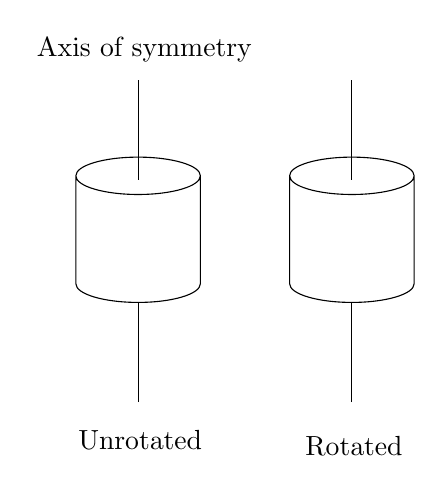
\begin{tikzpicture}[x=0.75pt,y=0.75pt,yscale=-1,xscale=1]
%uncomment if require: \path (0,300); %set diagram left start at 0, and has height of 300

%Shape: Can [id:dp6111663527038986] 
\draw   (154,122) -- (154,174) .. controls (154,178.97) and (140.57,183) .. (124,183) .. controls (107.43,183) and (94,178.97) .. (94,174) -- (94,122) .. controls (94,117.03) and (107.43,113) .. (124,113) .. controls (140.57,113) and (154,117.03) .. (154,122) .. controls (154,126.97) and (140.57,131) .. (124,131) .. controls (107.43,131) and (94,126.97) .. (94,122) ;
%Straight Lines [id:da6016989853853066] 
\draw    (124,124) -- (124,76) ;
%Straight Lines [id:da7742642520386162] 
\draw    (124,231) -- (124,183) ;
%Shape: Can [id:dp6333770541501842] 
\draw   (257,122) -- (257,174) .. controls (257,178.97) and (243.57,183) .. (227,183) .. controls (210.43,183) and (197,178.97) .. (197,174) -- (197,122) .. controls (197,117.03) and (210.43,113) .. (227,113) .. controls (243.57,113) and (257,117.03) .. (257,122) .. controls (257,126.97) and (243.57,131) .. (227,131) .. controls (210.43,131) and (197,126.97) .. (197,122) ;
%Straight Lines [id:da2230680788551479] 
\draw    (227,124) -- (227,76) ;
%Straight Lines [id:da2565843946616415] 
\draw    (227,231) -- (227,183) ;

% Text Node
\draw (125,249) node   [align=left] {Unrotated};
% Text Node
\draw (228,252) node   [align=left] {Rotated};
% Text Node
\draw (127,61) node   [align=left] {Axis of symmetry};


\end{tikzpicture}
    \caption{Symmetry of a cylinder}
    \label{fig:cylinder-rot}
\end{figure}
Mathematically, when we change our position of observation, it is equivalent to using a new, different reference frame and coordinate system, oriented differently from, and/or displaced relative to, the original. So a transformation can be viewed simply as a change of coordinate system, and this is often represented as a shifting from unprimed to primed coordinates. In QFT, \textbf{we will focus on passive transformation interpretation.}

\begin{example}
Consider the function 
\begin{equation}
g\left(x^{1}, x^{2}\right)=\left(x^{2}\right)^{2}
\end{equation}
if we have the following rorational transformation as
$$
\left[\begin{array}{l}
{x^{\prime 1}} \\
{x^{\prime 2}}
\end{array}\right]=\underbrace{\left[\begin{array}{cc}
{\cos \theta} & {\sin \theta} \\
{-\sin \theta} & {\cos \theta}
\end{array}\right]}_T\left[\begin{array}{l}
{x^{1}} \\
{x^{2}}
\end{array}\right]
\quad
\left[\begin{array}{l}
{x^{1}} \\
{x^{2}}
\end{array}\right]=\underbrace{\left[\begin{array}{ll}
{\cos \theta} & {-\sin \theta} \\
{\sin \theta} & {\cos \theta}
\end{array}\right]}_{T^{-1}=T^T}\left[\begin{array}{l}
{x^{\prime1}} \\
{x^{\prime2}}
\end{array}\right]
$$
we can express the function in the primed coordinate as:
$$
g=\left(x^{2}\right)^{2}=\left(x^{\prime 1} \sin \theta+x^{\prime 2} \cos \theta\right)^{2}=\left(x^{\prime 1}\right)^{2} \sin ^{2} \theta+\left(x^{\prime 2}\right)^{2} \cos ^{2} \theta+2 x^{\prime 1} x^{\prime 2} \sin \theta \cos \theta \neq\left(x^{\prime 2}\right)^{2}
$$
The transformed form of $g,$ represented by $g^{\prime}$, has the same value at the same physical point, but it is not the same form in terms of the primed coordinates as $g$ was in terms of the unprimed coordinates. But $f^{\prime},$ the transformed form of $f,$ did have the same form in terms of both sets of coordinates, and thus, we dropped the prime on $f$ on the RHS.

In spite of its non-symmetry under rotation, $g$ is symmetric under a different kind of Fransfort of the firc-symment ander founding $f$ the bynaced relative to the first along transformation, the translation to a coordinate system which is displaced relative to the first along the $x^{1}$ axis, i.e., $x^{1} \rightarrow x^{1}=x^{1}+$ constant $,$ or
$$
\left[\begin{array}{l}
{x^{\prime 1}} \\
{x^{\prime 2}}
\end{array}\right]=\left[\begin{array}{l}
{x^{1}} \\
{x^{2}}
\end{array}\right]+\left[\begin{array}{l}
{K} \\
{0}
\end{array}\right] \quad K=\text { constant }
$$
Substitution yields $g^{\prime}$ have the same form.
\end{example}
\begin{qt}
    From the example above, we can deduce the general rule that if a coordinate is missing in a given function, that function is invariant under a transformation solely in the direction of that coordinate (and also under multiplication of the coordiante by a constant).
\end{qt}
\textbf{\redp{So under any transformation of coordinate axes, the value at a physical point of every possible scalar function is invariant.}}
\subsection{Scalar are invariant, vectors are covariant}
\textbf{The scalar value at the point ( equal to the length of the position vector at that point) is the same in both systems, but the coordinate values are not.} For a 2D position vector in physical space, we have
$$
|x|=\left|x^{i}\right|=\sqrt{\left(x^{1}\right)^{2}+\left(x^{2}\right)^{2}}=\sqrt{\left(x^{\prime1}\right)^{2}+\left(x^{\prime2}\right)^{2}}=\left|x^{\prime i}\right|
$$
It is generally true of every vector $\mathbf{v},$ not just the position vector shown here, that its physical, measurable length (a scalar value) remains unchanged under any coordinate transformation, but its component values change. This is called covariance. Scalar values are invariant under coordinate transformation; vector components are \textbf{covariant}.
\begin{qt}
    General rule: if a function $h$ is not a function of the $j$th coordinate $x^j$, then h is symmetric under the transformation $x^{j} \rightarrow x^{j}+$ constant.
\end{qt}
\section{Symmetry in Classical Mechanics}
Recall that a Galilean transformation is
$$
\left[\begin{array}{c}
{x^{1}} \\
{x^{2}} \\
{x^{3}}
\end{array}\right] \rightarrow\left[\begin{array}{c}
{x^{11}} \\
{x^{\prime 2}} \\
{x^{3}}
\end{array}\right]=\left[\begin{array}{c}
{x^{1}-v^{1} t} \\
{x^{2}-v^{2} t} \\
{x^{3}-v^{3} t}
\end{array}\right]
$$
Newtonian mechanics is invariant under the Galilean transformation. But \textbf{Maxwell's eqs are not invariant under Galilean transformation. Instead, it is invariant under Lorentz transformation}
\begin{qt}
    \begin{equation}
\left[\begin{array}{c}
{x^{0}} \\
{x^{1}} \\
{x^{2}} \\
{x^{3}}
\end{array}\right] \rightarrow\left[\begin{array}{c}
{x^{\prime 0}} \\
{x^{\prime 1}} \\
{x^{\prime 2}} \\
{x^{\prime 3}}
\end{array}\right]=\left[\begin{array}{c}
{\gamma\left(x^{0}-\frac{v}{c} x^{1}\right)} \\
{\gamma\left(x^{1}-\frac{v}{c} x^{0}\right)} \\
{x^{2}} \\
{x^{3}}
\end{array}\right]=\underbrace{\left[\begin{array}{cccc}
{\gamma} & {-\gamma \frac{v}{c}} & {0} & {0} \\
{-\gamma \frac{v}{c}} & {\gamma} & {0} & {0} \\
{0} & {0} & {1} & {0} \\
{0} & {0} & {0} & {1}
\end{array}\right]}_{\Lambda}\left[\begin{array}{c}
{x^{0}} \\
{x^{1}} \\
{x^{2}} \\
{x^{3}}
\end{array}\right]
\label{lorentz-trans}
\end{equation}
where
$$
\gamma=\frac{1}{\sqrt{1-\frac{v^{2}}{c^{2}}}} \quad v=v^{1}
$$
\end{qt}
The index notation for Lorentz transformations is 
\begin{qt}
    \begin{equation}
x^{\prime \mu}=\Lambda^{\mu}{}_{v} x^{v} \quad V^{\prime \mu}\left(x^{\prime \alpha}\right)=\Lambda^{\mu}{}_{v} V^{v}\left(x^{\alpha}\right) \quad T^{\prime \mu v}\left(x^{\prime \alpha}\right)=\Lambda^{\mu}{}_{\delta} \Lambda^{v}{}_{\gamma} T^{\delta \gamma}\left(x^{\alpha}\right)
\end{equation}
Note that $\Lambda^{-1},$ the inverse of $\Lambda,$ can be obtained by taking $\mathbf{v} \rightarrow-\mathbf{v}$ since each coordinate system seems to be going in the opposite direction with respect to the other. $\Lambda^{-1}$ will transform $x^{\prime \mu}$ back into $x^{\mu}$.
\end{qt}
\bluep{Recall that the length of a vector in 3D is unchanged under a coordinate system transformation, 1.e., the length 1s a scalar and thus invariant. The same thing is true in 4D for four-vectors.}
$$
w_{\mu} w^{\mu}=w_{0} w^{0}+w_{1} w^{1}+w_{2} w^{2}+w_{3} w^{3}=w^{0} w^{0}-w^{1} w^{1}-w^{2} w^{2}-w^{3} w^{3}=\text { scalar invariant }
$$
\textbf{and that this is the same for any observer in any inertial coordinate system. This applies to any
vector, be it a position vector like $x^{\mu},$ the differential of position $d x^{\mu},$ the four-velocity $u^{\mu}$, the four potential $A^{\mu}$, the partial derivative $\partial^{\mu}$, or any other}.For instance,
$$
\frac{\partial}{\partial x^{\mu}} \frac{\partial}{\partial x_{\mu}}=\partial_{\mu} \partial^{\mu}=\frac{\partial}{\partial x^{0}} \frac{\partial}{\partial x^{0}}-\frac{\partial}{\partial x^{1}} \frac{\partial}{\partial x^{1}}-\frac{\partial}{\partial x^{2}} \frac{\partial}{\partial x^{2}}-\frac{\partial}{\partial x^{3}} \frac{\partial}{\partial x^{3}}=\text { scalar invariant derivative, }
$$
So if X represents a quantity, we have
$$
\frac{\partial}{\partial x^{\mu}} \frac{\partial}{\partial x_{\mu}}=\frac{\partial}{\partial x^{\prime \mu}} \frac{\partial}{\partial x_{\mu}^{\prime}} \rightarrow \frac{\partial}{\partial x^{\mu}} \frac{\partial}{\partial x_{\mu}} X=\frac{\partial}{\partial x^{\prime\mu}} \frac{\partial}{\partial x_{\mu}^{\prime}} X
$$
\subsection{Poincare transformation}
The most general transformation we could have in spacetime would comprise 1) a 4D translation(translating our coordinate axes in space, time, or both), 2) a rotation in space, and 3) a Lorentz transformation to a frame with different relative velocity. (We ignore reflection.)

The rotation in 3D is the same. It does allow us to rotate our 3D axes, however, so that the relative velocity between our original and transformed systems is along the $x^1$ axes of both. \textbf{This lets us use the Lorentz transformation in its simplest form (\ref{lorentz-trans})}. With this form we state the general transformation between coordinate systems, know as \redp{\textbf{Poincare transformation}} as
\begin{equation}
x^{\mu}=\Lambda_{\nu}^{\mu}\left(x^{\nu}+a^{\nu}\right) \quad a^{\nu}=\mathrm{constant} \text { four vector }
\label{poincare-trans}
\end{equation}

\subsection{Other kinds of symmetry}
Consider the Euler-Lagrange equation for a particle in Newtonian mechanics
$$
\frac{d}{d t}\left(\frac{\partial L}{\partial \dot{x}^{i}}\right)-\frac{\partial L}{\partial x^{i}}=0 \quad L=T-V \quad p_{i}=\frac{\partial L}{\partial \dot{x}^{i}}
$$
If the Lagrangian $L$ is not an explicit function of the spatial coordinate $x^i,$ then $\partial L / \partial x^{i}=0$ on the LHS above. Thus, the time derivative of $p_{i}$ is zero.
$$
\frac{d}{d t}\left(\frac{\partial L}{\partial \dot{x}^{i}}\right)=\frac{d p_{i}}{d t}=0 \quad \text { with } \frac{\partial L}{\partial x^{i}}=0 \quad \text { when } \quad L \neq L\left(x^{i}\right)
$$
Hence $p^i$ is constant and thus, conserved. This makes sense since the only source for spatial dependence in $L$ is the potential energy $V$. If we have no $V$ dependence on $x^i$, then there is no force in the $x^i$ direction, and momentum $p_i$ is constant.\textbf{Note this means the Lagrangian is symmtric.}

\redp{If the Lagrangian is symmetric in a coordinate, then the conjugate momentum for that coordiante is conserved.}

\section{Transformations in QFT}
\subsection{Spinor transformation}
For spinor, we seek a matrix which is four by four in spinor space and which represents what ha~pens to a spmor under a Lorentz transformation and/or a rotation of coordinates. That is, we seek D in
\begin{equation}
\psi^{\prime}\left(x^{\prime \mu}\right)=D \psi\left(x^{\mu}\right) \quad \frac{\text { with spinor indices }}{\text { written out }} \quad \psi_{\alpha}^{\prime}\left(x^{\prime \mu}\right)=D_{\alpha \beta} \psi_{\beta}\left(x^{\mu}\right)
\end{equation}
The spinor transformation under Lorentz and rotation transformation is
\begin{equation}
D=e^{-i(\mathbf{L} \mathbf{\Theta}+\mathbf{M} \mathbf{Q})} \quad L^{k}=-\frac{i}{2} \varepsilon_{i j}^{k} \gamma^{i} \gamma^{j}, \quad \Theta^{k}=\left(\theta^{1}, \theta^{2}, \theta^{3}\right), M^{k}=\frac{i}{2} \gamma^{0} \gamma^{k}, Q^{k}=\left(v^{1}, v^{2}, v^{3}\right)
\end{equation}
where $\Theta^{k}$ represents rotation angles of the primed system with respect to the unprimed system; $Q^k$ is a three vector of the boost velocities; and $\epsilon_{ij}{}^{k}$ is zero unless $i,j,k$ are all different, 1 if $ijk=123,231,312$, and -1 for the others.

Note that in formal mathematical language, the set of all possible Lorentz transformations (all possible v) is known as the Lorentz group. When the Lorentz group acts on the coordinate system, it changes what our spinors look like in the new system and this change is represented by $D$. So, \textbf{$D$ is called a representation of the Lorentz group.} It "represents" that group in spinor space.
\begin{qt}
    $\bar{\psi} \psi=$ world scalar $\quad \bar{\psi} \gamma^{\mu} \psi=$ transforms like four vector.
\end{qt}
\section{Lorentz Symmetry of the Lagrangian Density}
Lagrangian Density is symmetric under Lorentz transformation. We conclude this because of Einstein's postulate that the laws of nature (the field equation here) is invariant in form under Lorentz transformation. The Euler-Lagrange equation for fields, which is another form of the field equation, is a law of nature and must, therefore be invariant in form as well.

\section{Noether's Theorem}
There are other ways the Lagrangian density can be symmetric, for example
\begin{equation}
\phi \rightarrow \phi^{\prime}=\phi e^{-i \alpha}
\label{phase-trans}
\end{equation}
and for free scalar field, we have
$$
\mathcal{L}_{0}^{0}=\partial_{v} \underbrace{\phi^{r+} e^{-i \alpha}}_{\phi^{\dagger}} \partial^{v} \underbrace{\phi^{\prime} e^{i a}}_{\phi}-\mu^{2} \underbrace{\phi^{\prime} e^{-i \alpha}}_{\phi^{\dagger}} \underbrace{\phi^{\prime} e^{i \alpha}}_{\phi}=\mathcal{L}_{0}^{0}\left(\phi^{\prime\dagger}, \phi^{\prime}\right)
$$
\subsection{Internal and external symmetries}
Poincaré transformations (Lorentz plus $4 \mathrm{D}$ translation) and $3 \mathrm{D}$ rotations involve changes $\mathrm{t}$ to physical coordinates $x^{\mu}$ of our external world and are called \textbf{external transformations}.

Transformation like (\ref{phase-trans}) have nothing to do with $x^{\mu}$, but instead function in hidden spaces, behind the scene, like Hilbert or Fock space. They are called \textbf{internal transformation}.
\begin{qt}
   Noether's theorem in words: \textbf{ A symmetry in the Lagrangian density implies an associated quantity is conserved.}
   
   Mathematically:If the Lagrangian density $\mathcal{L}\left(\phi^{r}, \phi^{r}, \mu\right)$ is symmetric in form with respect to a transformation in $\phi^{r}$ which is a function of parameter $\alpha$,i.e., $\phi^{r}\left(x^{\mu}\right) \rightarrow \phi^{r}\left(x^{\mu}, \alpha\right)$ then the four current (using $\left.\phi^{r}\left(x^{\mu}, \alpha\right)\right)$
   \begin{equation}
j^{\mu}\left(\phi^{r}, \phi_{, \nu}^{r}\right)=\frac{\partial \mathcal{L}}{\partial \phi_{, \mu}^{r}} \frac{\partial \phi^{r}}{\partial \alpha} \quad(\text { sum on } r)
\end{equation}
bas zero four-divergence,$\partial_{\mu} j^{\mu}=0$. Thus, its zeroth component $j^0$ integrated over all the space is conserved, as is $q j^{0}$ integrated over all space, where $q$ is a constant.
\end{qt}
\subsection{Apply Noether's theorem to free scalar field}
$$
\frac{\partial \mathcal{L}_{0}^{0}}{\partial \phi_{\mu}}=\frac{\partial}{\partial \phi_{, \mu}}\left(\phi_{, \nu}^{\dagger} \phi^{\nu}-\mu^{2} \phi^{\dagger} \phi\right)=\frac{\partial}{\partial \phi_{\mu}}\left(\phi_{, \mu}^{\dagger} \phi^{\nu}\right)
=\frac{\partial \phi_{, \nu}^{\dagger}}{\partial \phi_{\mu}} \phi^{,\nu}+\phi_{, \nu}^{\dagger} \frac{\partial \phi^{,\nu}}{\partial \phi_{,\mu}}=\phi_{, \nu}^{\dagger} g^{\nu \mu}=\phi^{\dagger, \mu}
$$
$$
\frac{\partial \mathcal{L}_{0}^{0}}{\partial \phi^{\dagger}, \mu}=\frac{\partial}{\partial \phi^{\dagger}, \mu}\left(\phi_{, \nu}^{\dagger} \phi^{\nu}-\mu^{2} \phi^{\dagger} \phi\right)=\frac{\partial}{\partial \phi^{\dagger}}\left(\phi^{\dagger}, \phi^{,\nu}\right)=\frac{\partial \phi^{\dagger}_{, \nu}}{\partial \phi^{\dagger}_{, \mu}} \phi^{,\nu}=\delta_{v}^{\mu} \phi^{, v}=\phi^{,\mu}
$$
and
$$
\begin{array}{l}
{\frac{\partial \phi\left(x^{\eta}, \alpha\right)}{\partial \alpha}=\frac{\partial}{\partial \alpha} \phi\left(x^{\eta}\right) e^{-i \alpha}=-i \phi\left(x^{\eta}\right) e^{-i \alpha}} \\
{\frac{\partial \phi^{\dagger}\left(x^{\eta}, \alpha\right)}{\partial \alpha}=\frac{\partial}{\partial \alpha} \phi^{\dagger}\left(x^{\eta}\right) e^{i \alpha}=i \phi^{\dagger}\left(x^{\eta}\right) e^{i \alpha}}
\end{array}
$$
Using the relation above, we have
$$
j^{\mu}\left(\phi^{r}, \phi^{r}_{,v}\right)=i\left(\phi^{,\mu}\left(x^{\eta}\right) \phi^{\dagger}\left(x^{\eta}\right)-\phi^{\dagger, \mu}\left(x^{\eta}\right) \phi\left(x^{\eta}\right)\right)
$$
This is identical to the scalar four-current.\redp{The expectation value ( expected measurement) of a conserved operator is conserved. If the state measured is in an eigenstate, any measurement at any time will yield the same eigenvalue}.
\section{Symmetry, Gauges, and Gauge theory}
\begin{itemize}
    \item \textbf{Gauge invariance }(or gauge symmetry) is the property of a field theory in which different configurations of the underlying fundamental, but unobservable, field(s) result in identical observable properties.
    \item the unobservable field, often a potential field, is called the\textbf{ gauge field}.
    \item A gauge transformation changes the gauge field from one configuration to another. \redp{Each different configuration of the gauge field is a different gauge.}
    \item A theory have gauge invariance (symmetry) is called a gauge theory.
\end{itemize}
\redp{\textbf{We can also say that a gauge theory is a type of field theory in which the Lagrangian ( density) is invariant under a continuous (not discrete) transformation.}}
\section{A Solved Exercise}
\textbf{Problem 14.} Show that the total (not density) 3-momentum $k^{i}$ for free scalars is conserved. Use our knowledge that the conjugate momentum for $x^{i}$ is $k_{i}$, the total (not density) 3 -momentum (expressed in covariant components), and it is conserved if $L$ is symmetric (invariant) under the coordinate translation transformation $x^{t} \rightarrow x^{1}=x^{t},$ where $\alpha^{t}$ is a constant $3-$ vector. Then, show the same result via commutation of the three-momentum operator.

\textbf{Solution}
The Lagrangian density is $\mathcal{L}_{0}^{0}=\phi_{, \mu}^{\dagger} \phi^{\mu}-\mu^{2} \phi^{\dagger} \phi .$ We must integrate this over all volume to get the total Lagrangian $L$. If $k_{i}$ is conserved, then of course, so is $k^{i}$. So, we need to show $L$ is invariant under $x^{i} \rightarrow x^{i}=x^{i}+\alpha^{i}$
$$
\phi=\sum_{\mathbf{k}} \frac{1}{\sqrt{2 V a_{\mathbf{k}}}}\left(a(\mathbf{k}) e^{-i k_{\mu} x^{\mu}}+b^{\dagger}(\mathbf{k}) e^{i k_{\mu} x^{\mu}}\right) \quad \phi^{\dagger}=\sum_{\mathbf{k}} \frac{1}{\sqrt{2 V a_{k}}}\left(b(\mathbf{k}) e^{-i k_{\mu} x^{\mu}}+a^{\dagger}(\mathbf{k}) e^{i k_{\mu} x^{\mu}}\right)
$$
$$
\begin{array}{l}
{\phi_{s}, \mu=\sum_{\mathbf{k}} \frac{i k_{\mu}}{\sqrt{2 V \omega_{\mathbf{k}}}}\left(-a(\mathbf{k}) e^{-i k_{\mu} x^{\mu}}+b^{\dagger}(\mathbf{k}) e^{i k_{\mu} x^{\mu}}\right)} \\
{\phi^{, \mu}=\sum_{\mathbf{k}} \frac{i k^{\mu}}{\sqrt{2 V a_{k}}}\left(-a(\mathbf{k}) e^{-i k_{\mu} x^{\mu}}+b^{\dagger}(\mathbf{k}) e^{i k_{\mu} x^{\mu}}\right)}
\end{array}
$$
$$
\begin{aligned}
\phi^{\dagger}_{z \mu} \phi^{z}=\sum_{\mathbf{k}} \sum_{\mathbf{k}^{*}} \frac{-1}{2 V} \frac{k_{\mu} k^{* \mu}}{\sqrt{\omega_{\mathbf{k}} \omega_{\mathbf{k}^{*}}}}\left(b(\mathbf{k}) a\left(\mathbf{k}^{*}\right) e^{-i k_{A} x^{\mu}} e^{-i k_{A}^{*} x^{\mu}}-b(\mathbf{k}) b^{\dagger}\left(\mathbf{k}^{*}\right) e^{-i k_{\mu} x^{\mu}} e^{i k_{\mu} x^{\mu}}\right.\\
-a^{\dagger}(\mathbf{k}) a\left(\mathbf{k}^{*}\right) e^{i k_{\mu} x^{\mu}} e^{-i k_{\mu} x^{\mu}}+a^{\dagger}(\mathbf{k}) b^{\dagger}\left(\mathbf{k}^{*}\right) e^{i k_{\mu} x^{\mu}} e^{i k_{\mu} x^{\mu}}
\end{aligned}
$$
For $k_{i}=-k^*_i$, we have $$
\left.k_{\mu} k^{* \mu}=\omega_{\mathbf{k}}^{2}+k_{i} k^{*i}=\omega_{\mathbf{k}}^{2}+k_{i}\left(-k^{i}\right)=\omega_{\mathbf{k}}^{2}+k_{i} k_{i}=k_{\mu} k_{\mu}\right.
$$
$$
\int \phi^{\dagger}_{,\mu} \phi^{, \mu} d V=\sum_{k} \frac{-1}{2 \omega_{k}}\left(\begin{array}{c}
{k_{\mu} k_{\mu} e^{-i 2 \omega_{k} t} b(\mathbf{k}) a(-\mathbf{k})-k_{\mu} k^{\mu} b(\mathbf{k}) b^{\dagger}(\mathbf{k})} \\
{-k_{\mu} k^{\mu} a^{\dagger}(\mathbf{k}) a(\mathbf{k})+k_{\mu} k_{\mu} e^{i 2 \omega_{k} t} a^{\dagger}(\mathbf{k}) b^{\dagger}(-\mathbf{k})}
\end{array}\right)
$$
Similarly,
$$
\int \mu^{2} \phi^{\dagger} \phi d V=-\sum_{\mathbf{k}} \frac{\mu^{2}}{2 \omega_{\mathbf{k}}}\left(e^{-i 2 \omega_{\mathbf{k}} t} b(\mathbf{k}) a(-\mathbf{k})+b(\mathbf{k}) b^{\dagger}(\mathbf{k})+a^{\dagger}(\mathbf{k}) a(\mathbf{k})+e^{i 2 \omega_{\mathbf{k}} t} a^{\dagger}(\mathbf{k}) b^{\dagger}(-\mathbf{k})\right)
$$
It is easy to show that, after the transformation the forms of $\int \mu^{2} \phi^{\dagger} \phi d V$ and $\int \phi^{\dagger}_{,\mu} \phi^{, \mu} d V$ will not change, so L is symmetric in some coordinate, then the conjugate momentum of that coordinate is conserved. $k_{i}$, the particle(s) 3 -momentum is the conjugate momentum of $x^{i} .$ Thus, $k_{i}$, is conserved.

Also
$$
H=\sum_{\mathbf{k}} \omega_{\mathbf{k}}\left(N_{a}(\mathbf{k})+N_{b}(\mathbf{k})\right) \quad \mathbf{P}=\sum_{\mathbf{k}} \mathbf{k}\left(N_{a}(\mathbf{k})+N_{b}(\mathbf{k})\right) \rightarrow[H, \mathbf{P}]=0 \quad\left(\begin{array}{ll}
{\text { because all number }} \\
{\text { operators commute }}
\end{array}\right)
$$
Thus $\mathbf{P}$ is conserved for the free Hamiltonian.
\chapter{Interactions: The Underlying Theory}
\section{Interactions in RQM}
\subsection{Maxwell's equation with sources}
If we include the charge density and current density into Maxwell's equation, we have
\begin{equation}
\begin{aligned}
&\nabla \cdot \mathbf{E}=\rho_{charge}\\
&\nabla \times \mathbf{B}-\frac{\partial \mathbf{E}}{\partial t}=\mathbf{j}_{charge}\\
&\nabla \cdot \mathbf{B}=0\\
&\vec{\nabla} \times \mathbf{E}=-\frac{\partial \mathbf{B}}{\partial t}
\end{aligned}
\end{equation}
By introducing the potentials $\Phi$ and $\mathbf{A}$, where 
$$
\mathbf{B}=\nabla \times \mathbf{A}, \quad \mathbf{E}=-\nabla \Phi-\frac{\partial \mathbf{A}}{\partial t}
$$
one gets
\begin{equation}
\begin{aligned}
&-\nabla \frac{\partial \Phi}{\partial t}-\nabla(\nabla \cdot \mathbf{A})=\rho_{charge}\\
&\frac{\partial^{2} \mathbf{A}}{\partial t^{2}}-\nabla^{2} \mathbf{A}+\nabla \frac{\partial \Phi}{\partial t}+\nabla(\nabla\cdot\mathbf{A})=\mathbf{j}_{charge}
\end{aligned}
\end{equation}
Rewrite the equations above in terms of 4-potential and 4-current $-ej^{\mu}$=($\rho_{charge},\mathbf{j}_{charge}$):
\begin{equation}
    \partial^{\alpha}\partial_{\alpha}A^{\mu}(x)-\partial^{\mu}\left(\partial_{\nu}A^{\nu}(x)\right)=-ej^{\mu}(x)
\end{equation}
Using Lorenz gauge condition, we have
\begin{qt}
\begin{equation}
    \partial^{\alpha}\partial_{\alpha}A^{\mu}(x)=-ej^{\mu}
    \label{maxwell-4D-interaction-eqn}
\end{equation}
\end{qt}
\subsection{The classical Lagrangian density for interaction}
The full electromagnetic Lagrangian(density), including interactions, must give rise to (\ref{maxwell-4D-interaction-eqn}) when substituted into the Euler-Lagrange field equation:
$$
\frac{\partial}{\partial x^{v}}\left(\frac{\partial \mathcal{L}}{\partial \phi_{v}^{n}}\right)-\frac{\partial \mathcal{L}}{\partial \phi^{n}}=0, \quad \text { with } \quad \phi^{n}=A_{\mu} ; \mathcal{L}=\mathcal{L}^{e / m}
$$
One can prove that the full electromagnetic field classical Lagrangian is
\begin{qt}
\begin{equation}
\mathcal{L}^{e / m}=\underbrace{-\frac{1}{2}\left(\partial_{v} A_{\mu}(x)\right)\left(\partial^{v} A^{\mu}(x)\right)}_{\mathcal{L}_{0}^{e / m}}+ \underbrace{e j^{\mu}(x) A_{\mu}(x)}_{\mathcal{L}_{1}^{e / m}}
\label{full-electromagnetic-field-classical-lagrangian}
\end{equation}
where "0" and "1" subscripts denote the free and interaction parts, respectively, of the Lagrangian.
\end{qt}
\subsection{Electromagnetic Interactions in RQM}
Relations (\ref{maxwell-4D-interaction-eqn}) and (\ref{full-electromagnetic-field-classical-lagrangian}) hold for classical electromagnetism where $-ej^{\mu}$ is the classical electric charge 4-current. \textbf{In quantization, we assume the quantum form of the Lagrangian (density or total) is the same as the classical, and thus, so would be the resulting wave equation.} In RQM, we would then consider $A^{\mu}$ to represent the quantum photon state (ket, wave function). Thus, (\ref{full-electromagnetic-field-classical-lagrangian}) represents the RQM electromagnetic Lagrangian. But then, \bluep{how should one interpret $-ej^{\mu}$?} In Chap.3, we saw that the probability 4-current for an electron in RQM, where $\psi_{state}$ represents the electron wave function state, is
$$
j^{\mu}=(\rho, \mathbf{j})=\bar{\psi}_{\text {state}} \gamma^{\mu} \psi_{\text {state}} \quad \text { where } \partial_{\mu} j^{\mu}=0
$$
\redp{It seems natural to assume charge density varies directly with probability density.} Thus, we can assume
\begin{equation}
-e j^{\mu}=-e \bar{\psi}_{\text {state}} \gamma^{\mu} \psi_{\text {state}}
\label{electron-4-current-state}
\end{equation}
where the total charge of the electron would be
$$
-e \int j^{0} d^{3} x=-e
$$
Using (\ref{maxwell-4D-interaction-eqn}),(\ref{full-electromagnetic-field-classical-lagrangian}), and(\ref{electron-4-current-state}), we can then represent the \textbf{\redp{RQM interaction wave equation for a photon}} as
\begin{equation}
\partial^{\alpha} \partial_{\alpha} A_{\text {stale}}^{\mu}=-e \bar{\psi}_{\text {state}} \gamma^{\mu} \psi_{\text {state}}
\label{RQM-photon-interaction-wave-eqn}
\end{equation}
with the corresponding \textbf{\redp{RQM e/m interaction Lagrangian for a photon}} as
\begin{equation}
\mathcal{L}^{e / m}=\underbrace{-\frac{1}{2}\left(\partial_{v} A_{\mu,state}\right)\left(\partial^{v} A_{\text {state }}^{\mu}\right)}_{\mathcal{L}_0^{e/m}}+\underbrace{e \bar{\psi}_{\text {state}} \gamma^{\mu} \psi_{\text {state}} A_{\mu,state}}_{\mathcal{L}_I^{e/m}}
\label{RQM-em-interaction Lagrangian-for-photon}
\end{equation}
\redp{\textbf{(\ref{RQM-photon-interaction-wave-eqn}) governs the behavior of a photon ($A^{\mu}_{state}$) in the presence of an electron ($\psi_{state}$)}}.
\subsection{The electromagnetic interaction Dirac equation}
We now develop the full Dirac equation describing the electron interacting with a photon. To this end, consider that $\mathcal{L}_{0}^{e / m}$ of (\ref{RQM-em-interaction Lagrangian-for-photon}) represents the free photon part of the full e/m Lagrangian. If we assume $\mathcal{L}_{1}^{e / m}$ represents the e/m interaction part for both the photon and the electron, then \textbf{\redp{we need only add the free electron contribution to (\ref{RQM-em-interaction Lagrangian-for-photon}) to get a Lagrangian containing all terms relevant to photons, electrons, and interactions between them.}} Since from Chap 3
$$
\mathcal{L}_{0}^{1 / 2}=\bar{\psi}_{\text {state}}\left(i \gamma^{\mu} \partial_{\mu}-m\right) \psi_{\text {state}}
$$
Thus, the \textbf{full e/m Lagrangian} is
\begin{equation}
\mathcal{L}^{1 / 2,1}=\underbrace{-\frac{1}{2}\left(\partial_{v} A_{\mu,state}\right)\left(\partial^{v} A_{\text {state}}^{\mu}\right)}_{\mathcal{L}_{0}^{1}=\mathcal{L}_{0}^{e / m}}+\underbrace{\bar{\psi}_{\text {state}}\left(i \gamma^{\mu} \partial_{\mu}-m\right) \psi_{\text {state}}}_{\mathcal{L}_{0}^{1 / 2}}+\underbrace{e \bar{\psi}_{\text {state}} \gamma^{\mu} \psi_{\text {state}} A_{\mu,state}}_{\mathcal{L}_{1}^{1 / 2,1}=\mathcal{L}_{1}^{e/m}}
\label{full-e/m-lagrangian}
\end{equation}
To find the interaction form of the Dirac equation, we use (\ref{full-e/m-lagrangian}) in Euler-Lagrange equation with $\phi^{n=1}=\bar{\psi}$. The result is
\begin{qt}
\begin{equation}
\left(i \gamma^{\mu} \partial_{\mu}-m\right) \psi_{\text {state }}=-e \gamma^{\mu} \psi_{\text {state }} A_{\mu,state}
\label{full-Dirac-eqn}
\end{equation}
As an aside, using (\ref{full-e/m-lagrangian}) with $\phi^{n=2}=\psi$ results in the adjoint full Dirac equation.
\end{qt}

\begin{mybox}
A this point, some might be concerned that we have used the Lagrangian density methodology, which is normally reserved for quantum and classical fields, to develop the full Dirac equation for quantum states (corresponding to particles, not fields).One would expect to use the
total Lagrangian L (integration of $\mathcal{L}$ over all space) instead of $\mathcal{L}$, since (\ref{full-Dirac-eqn}) is a wave equation for interacting states, not fields.

However, even in the context of $1^{\text {st }}$ (particle) and $2^{\text {nd }}$ (field) quantization as we have come to understand them, the issue is not such a big one. This is because we did not employ commutation relations for fields $A^{\mu}$ and $\psi,$ analogous to Poisson bracket relations, in the above development, It is the adth $^{\mu} A^{\mu}$ and $\psi,$ analogous to Poisson bracket relations, in the above development, \textbf{it is the adoption of commutation relations for those fields that turns them into creation and destruction operators quantum mechanically.} We did not do that, so $A^{\mu}$ and $\psi$ remain as states, not quantum fields, in the above treatment. Of course, for RQM, we would still have commutation relations for dynamical variable gnerators, such as $p_{x}$ and $X_{1}$, though we would not have them for $A^{\mu}$ and $\psi$
\end{mybox}
\section{Interactions in QFT}
Our interacting spinor field and photon wave equations in the Heisenberg picture should simply be the following for fields,
\begin{equation}
\partial^{\alpha} \partial_{\alpha} A^{\mu}=-e \bar{\psi} \gamma^{\mu} \psi
\label{fields-interaction-wave-eqn-1}
\end{equation}
\begin{equation}
\left(i \gamma^{\mu} \partial_{\mu}-m\right) \psi=-e \gamma^{\mu} A_{\mu} \psi
\label{fields-interaction-wave-eqn-2}
\end{equation}
where the order of $\psi$ and $A_{\mu}$ in the equations above is unimportant, even though they are operators, since \redp{different type fields commute}. The associated Lagrangian for the $\psi$ and $A^{\mu}$ operator fields is
\begin{equation}
\mathcal{L}^{1 / 2,1}=\underbrace{-\frac{1}{2}\left(\partial_{v} A_{\mu}\right)\left(\partial^{v} A^{\mu}\right)}_{\mathcal{L}_{0}^{1}}+\underbrace{\bar{\psi}\left(i \gamma^{a} \partial_{\alpha}-m\right) \psi}_{\mathcal{L}_0^{1/2}}+\underbrace{e \bar{\psi} \gamma^{\mu} A_{\mu} \psi}_{\mathcal{L}_{I}^{1 / 2,1}}
\end{equation}

Modern day computers can help in providing numerical solutions to these equations, but early researchers in QFT did not have such things. Also, the route those researchers did take provides considerable insight into the inner workings of the theory. That route, for the QFT e/m interaction theory known as \textbf{quantum electrodynamics (QED)}, was forged in large part by Richard Feynman, Freeman Dyson, Julian Schwinger, and Sin-Itiro Tomonaga. It involves two things,
\begin{itemize}
    \item perturbation theory, and
    \item a trick known as the Interaction picture
\end{itemize}
\begin{qt}
The expectation value for any quantum field, including spinor and vector fields, is zero.
\end{qt}

\section{Interaction Picture}
It turns out that a third picture, the Interaction Picture (I.P.) is easier to use for interactions in
QFT. For one reason, it facilitates use of perturbation theory in place of trying to solve the coupled, non-linear, partial differential equations (\ref{fields-interaction-wave-eqn-1}) and (\ref{fields-interaction-wave-eqn-2}).

Additionally, the LP. allows us to analyze interacting fields using all the results of our free QFT development.

\underline{Breaking the Hamiltonian into Free and Interaction Parts}
The Hamiltonian (total, not density) for e/m interactions in the (Schrödinger Picture) S.P. can be expressed, from the Lagrangian density (\ref{full-e/m-lagrangian}) and the Legendre transformation, as (with $\phi^{r}$ generically representing any quantum field)
\begin{equation}
\underbrace{H^{S}}_{H}=\underbrace{H^{1 / 2,1}}_{\text {just e/m }}=\underbrace{\int\left(\pi_{r} \dot{\phi}^{r}-\mathcal{L}_{0}^{1}-\mathcal{L}_{0}^{1 / 2}\right) d^{3} x}_{H_{0}^{S}=H_{0}(\text { free part })}-\underbrace{\int \mathcal{L}_{I}^{1 / 2,1} d^{3} x}_{H_{I}^{S}(\text { interaction part })}
\end{equation}
Thus,$H=H_{0}+H_{I}^{S}$. Note, for future reference, that for all cases  $\mathcal{H}_{I}=-\mathcal{L}_{I}$ and $ H_{I}=-L_{I}$.

\underline{Using only the free part of the Hamiltonian to transform to the interaction picture}

The transformation from the S.P. to the I.P. is
\begin{equation}
    U_{0}=e^{-i H_{0} t}
\end{equation}
where $U_0$ is a unitary operator, where
\begin{equation}
U_{0}^{\dagger}|\Psi\rangle_{S}=|\Psi\rangle_{I}
\end{equation}
and where subscripts "S" and "I" on generic states $|\Psi\rangle$ indicate the S.P. and I.P, respectively. For operators, where superscripts "S" and "I" represent the S.P. and I.P., respectively,
\begin{equation}
U_{0}^{\dagger} \mathcal{O}^{S} U_{0}=\mathcal{O}^{I}
\end{equation}

\underline{Parts of the Hamiltonian expressed in the I.P.}

For the free part of the Hamiltonian operator $H_{0}=H_{0}^{S},$ we see that
\begin{equation}
H_{0}^{I}=U_{0}^{\dagger} H_{0}^{S} U_{0}=U_{0}^{\dagger} H_{0} U_{0}=e^{i H_{0} t} H_{0} e^{-i H_{0} t}=H_{0} e^{i H_{0} t} e^{-i H_{0} t}=H_{0}
\end{equation}
because $H_{0}$ commutes with itself. Thus,
\begin{equation}
H_{0}=H_{0}^{S}=H_{0}^{I}
\end{equation}
\bluep{this equality generally does not hold for the interaction part:}
$$
H_{I}^{I}=U_{0}^{\dagger} H_{I}^{S} U_{0} \neq H_{I}^{S}
$$
and thus, we will represent the interaction picture Hamiltonian as
\begin{equation}
H^{I}=H_{0}+H_{I}^{I}
\end{equation}
\subsection{Equations of Motion in the I.P.}
$$
\frac{d \mathcal{O}^{l}}{d t}=\frac{d}{d t}\left(U_{0}^{+} \mathcal{O}^{s} U_{0}\right)=\frac{d U_{0}^{\dagger}}{d t} \mathcal{O}^{s} U_{0}+\underbrace{U_{0}^{\dagger} \frac{\partial \mathcal{O}^{S}}{\partial t} U_{0}}_{\text {defined }=\frac{\partial \mathcal{O}^{I}}{\partial t}}+U_{0}^{\dagger} \mathcal{O}^{s} \frac{d U_{0}}{d t}=
$$
$$
\frac{d e^{i H_{0} t}}{d t} \mathcal{O}^{S} e^{-i H_{0} t}+e^{i H_{0} t} \mathcal{O}^{S} \frac{d e^{-i H_{0} t}}{d t}+\frac{\partial \mathcal{O}^{I}}{\partial t}=i H_{0} \underbrace{e^{i H_{0} t} \mathcal{O}^{S} e^{-i H_{0} t}}_{\mathcal{O}^{I}}-\underbrace{e^{i H_{0} t} \mathcal{O}^{S} e^{-i H_{0} t}}_{\mathcal{O}^{I}} i H_{0}+\frac{\partial \mathcal{O}^{I}}{\partial t}
$$
or
\begin{qt}
\begin{equation}
\frac{d \mathcal{O}^{I}}{d t}=-i\left[\mathcal{O}^{I}, H_{0}\right]+\frac{\partial \mathcal{O}^{I}}{\partial t}
\end{equation}
\end{qt}
where the last term is zero in this note, because we only deal with operators for which $\partial \mathcal{O}^{S} / \partial t=0$. \redp{Thus, the equation of motion for operators in the I.P. depends only on the free part of the Hamiltonian.}

The \underline{I.P. equation of motion for states is}
\begin{equation}
i \frac{d}{d t}|\Psi\rangle_{I}=H_{I}^{I}|\Psi\rangle_{I}
\end{equation}
\redp{and hence, the equation of motion for states in the I.P. depends only on the interaction part of the Hamiltonian.}

\underline{The I.P. equation of motion for expectation values is}
\begin{equation}
\frac{d \overline{\mathcal{O}}}{d t}={}_{I}\left\langle\Psi\left|\left(-i\left[\mathcal{O}^{I}, H^{I}\right]+\frac{\partial \mathcal{O}^{I}}{\partial t}\right)\right| \Psi\right\rangle_{I}
\end{equation}
\end{document}
